\chapter{related work}
\label{chp:2_literature}

In this chapter, related studies are given in detail. Firstly, the concept of adversarial examples and the types of adversarial examples are explained briefly. Then, spatially transformed adversarial examples are explained in detail.
\section{Adversarial Examples}

The concept of adversarial examples were introduced by Szegedy et al.~\cite{szegedy2013intriguing}. They found that adding small calculated perturbances to the input image is able to change the decision of the target classifier (deep neural network) without affecting the decision human observers. Even though the perturbation is small, it can be easily noticed by human observers by "visual noise" instead of semantically meaningful patterns. Since this intriguing property of neural networks has security implications in the production setting, it is often called as adversarial attacks. For example, websites are using Completely Automated Public Turing Tests to Tell Computers and Humans Apart (CAPTCHA) to prevent web scrapers and spiders from automatically reaching their content. A widely used CAPTCHA is asking to select the images that is from a specific class such as "bicycle" or "crossroad" among the provided images. A human can effortlessly detect the suitable images while web scrapers need to use DNNs to classify each image and select the correct ones. Recent CAPTCHAs has extended this setup by adding adversarial perturbations to the provided images to prevent DNNs from automatically selecting the correct images. In Figure \ref{fig:googlecaptcha}, a recent CAPTHCA from Google is shown where it is asked to select the images that contains "cars". Normally, a trained DNN could be used to classify images and to select the images whose output is the class "car" to pass the test. However, there is a noticeable adversarial noise added to the images to fool the DNN and to prevent the scraper from passing the test.
\begin{figure}[t]
    \centering
    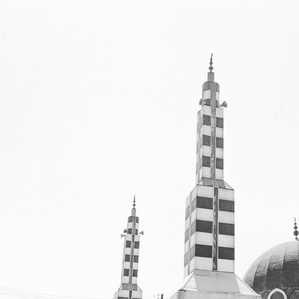
\includegraphics[width=0.4\linewidth]{captchas/1.png}
    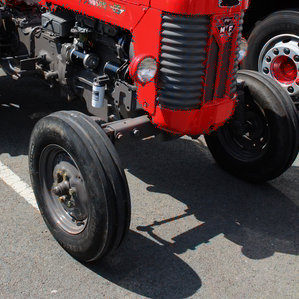
\includegraphics[width=0.4\linewidth]{captchas/2.png}
    \caption{Two CAPTCHA examples from Google where adversarial examples are used to fool web scrapers and spiders that are using automatic image classifiers such as DNNs.}\label{fig:googlecaptcha}
\end{figure}

Adversarial attacks can be classified as white-box and black-box depending on whether the attacker could reach the neural network parameters and gradients or not, respectively. Also, they can be classified as targeted or untargeted attacks. In targeted attack setup, there exists a particular class that attacker tries to modify the input image to have the attacked neural network to output that particular class and considered successful (or fooled the network) if the network outputs the target class when fed with the modified adversarial example. On the other hand, in the untargeted attack setting the attacker modifies the image to prevent the neural network from deciding the true class, which is the ground truth label of the input image and considered successful if the network outputs a class other than the true class label. In this thesis, targeted white-box attack setup is used. Other than the decision of the target network, there is often a magnitude constraint to the perturbation made and \(\mathcal{L}_p\) norms are widely used to measure the magnitude of the added perturbation. Adversarial attacks can be formally defined as a constrained optimization problem where the attacker tries to maximize a loss function by perturbing the input while the magnitude of the perturbation is constrained. Generally, the adversarial loss is the loss that is minimized throughout the training process. In most general form, the optimization process can be formulated as Equation \ref{eqn:advattackeqn}

\begin{equation}
    \label{eqn:advattackeqn}
    \underset{\|\delta\| \leq \epsilon}{\operatorname{maximize}} \ell\left(h_{\theta}(x+\delta), y\right)
\end{equation}

The equation simply indicates that the adversary is aiming to maximize a loss function of the adversarial image and the target label with the norm of the perturbation is upper bounded by \(\epsilon\). In the untargeted attack setup, the function is a single argument function of the adversarial image.

Since naively trained models are vulnerable to adversarial perturbations, the concept of adversarial training is introduced~\cite{madry2017towards}. In adversarial training, the datapoints are sampled from both original training set and on-the-fly generated adversarial attacks to the model that is being trained. Although the training time is significantly increased since adversarial example generation needs at least one forward and backward pass on the model, this method has been shown to increase the adversarial robustness of the trained model. There are several methods for adversarial example generation. The most widely used methods are explained in Section \ref{section:methods}.

\section{Adversarial Example Generation Methods}\label{section:methods}


\subsection{Fast Gradient Sign Method}

Goodfellow et al.\cite{goodfellow2014explaining} found that the fastest method of generating adversarial examples with \(l_\infty\) norm constraint by using the sign of gradient of the loss with respect to the input instead of the values of the gradient, named Fast Gradient Sign Method~(FGSM). The formal equation of the adversarial image generation process is shown in Equation \ref{eq:fgsm}

\begin{equation}
    \label{eq:fgsm}
    x_{adv} = x + \epsilon * \text{sign}(\bigtriangledown_{x}J(x,y))
\end{equation}

According to Goodfellow et al., this method works even when \(\epsilon\) is too small since the deep neural networks are actually linear in small local epsilon neighborhood of the input point. This method is generally used as a fast and easy to compute baseline in most works.

After FGSM, many sophisticated methods have been proposed for adversarial example generation with \(\mathcal{L}_p\) norm constraints. The most prominent and widely used algorithms are Projected Gradient Descent~(PDG) and Carlini \& Wagner method (C\&W) along with FGSM.

\subsection{Basic Iterative Method \& Projected Gradient Descent}
Basic Iterative Method~(BIM)~\cite{kurakin2018adversarialphys} can be simply thought as the iterative version of FGSM except that at each iteration, the adversarial example is clipped to the \(\epsilon\) neighborhood of the benign datapoint. This has found to be an useful heuristic since it allows generating more successful examples in terms of fooling rate without requiring significant computational budget.

Projected Gradient Descent~(PGD) \cite{madry2017towards} is very similar to BIM except that at each iteration projection operation instead of clipping is used to pull the adversarial example back to the \(\mathcal{L}_p\) ball around the original datapoint if necessary so that the \(\mathcal{L}_p\) constraint is satisfied througout the adversarial example generation process. This method is found to provide better robustness for the models trained with adversarial training than FGSM when training. The iteration steps of PGD and BIM for adversarial example generation is formalized in Equation~\ref{eq:bim} and Equation~\ref{eq:pgd}, respectively. This process repeats until the attack is successful or maximum iteration number is reached.

\begin{equation}
    \label{eq:bim}
    v^{i+1}=\operatorname{Clip}_{\epsilon}\left\{v^{i}+\alpha \operatorname{sign}\left(\nabla_{x+v^{i}} J\left(x+v^{i}, y\right)\right)\right\}
\end{equation}

\begin{equation}
    \label{eq:pgd}
    v^{i+1}=\operatorname{Project}_{\epsilon}\left\{v^{i}+\alpha \operatorname{sign}\left(\nabla_{x+v^{i}} J\left(x+v^{i}, y\right)\right)\right\}
\end{equation}


\subsection{Carlini \& Wagner Attack}
Carlini \& Wagner~\cite{carlini2017towards} attack is an iterative method for generating adversarial examples. It uses reformulation of the constrainted optimization objective so that the constraints are naturally satisfied without requiring an explicit step for clipping or projecting the adversarial example in the \(\mathcal{L}_p\) ball. The optimization process is formulated in Equation~\ref{eq:cw} and Equation~\ref{eq:cw2}

\begin{equation}
    \label{eq:cw}
    \operatorname{minimize}\left\|\frac{1}{2}(\tanh (w)+1)-\boldsymbol{I}\right\|_{2}^{2}+c \cdot f\left(\frac{1}{2}(\tanh (w)+1)\right)
\end{equation}

where

\begin{equation}
    \label{eq:cw2}
    F(m)=\max \left(\max _{i \neq t}\left(Z(m)_{i}\right)-Z(m)_{t}, \kappa\right)
\end{equation}

where \(\kappa\) denotes the target confidence for the adversarial example, which is the aimed score difference between the target class and the non-target class with the highest score.



\section{Colorspaces}
In most image processing tasks, standard RGB colorspace is used, where R, G, B denotes the Red, Blue, Green components of the image. However, it is incompatible with Human Visual System (HVS) so the need for HVS compatible (perceptual) colorspaces arises for the tasks concerning HVS such as lossy visual media compression where the media is compressed to reduce the size without affecting the perceived output. In this thesis, the perceptual colorspaces YUV, \(YC_{b}C_{r}\) and CIELAB are used.

\subsection*{YUV and YCbCr}
The \(YC_{b}C_{r}\) model defines a luminance component (Y) and two chrominance components \(C_{b}, C_{r}\) to specify color. \(YC_{b}C_{r}\) is a colorspace that is used in digital photography and visual media compression. In this space, luminance (brightness) and chrominance (color) is separated according to human visual perception. Y dimension of the space is the luminance information, or simply a grayscale representation of the image. \(C_b\) and \(C_r\) dimensions are the blue-difference and red-difference chroma components, respectively. The relation between RGB space and \(YC_{b}C_{r}\) space is modeled as Equation~\ref*{eq:rgbycbcr}, which is a set of linear equations defined in ITU-T H.273~\cite{hamilton2004jpeg};

\begin{align}
    \label{eq:rgbycbcr}
    \begin{split}
        Y   & = 0.299 R+0.587 G+0.114 B                   \\
        C_b & = 128-(0.168736 R)-(0.331264 G)+(0.5 B)     \\
        C_r & = 128+(0.5 R)-(0.418688 G)-(0.081312 B)     \\
        R & = Y+1.402(C_{r}-128)                        \\
        G & = Y-0.344136(C_{b}-128)-0.714136(C_{r}-128) \\
        B & = Y+1.772C_b-128
    \end{split}
\end{align}

YUV is often considered as the analog counterpart of \(YC_{b}C_{r}\). There is no significant difference between YUV and \(YC_{b}C_{r}\) except for the scaling of chrominance components to the range 0-255 for \(YC_{b}C_{r}\) so that they can be represented as unsigned integers while chrominance values can be negative in YUV colorspace. For that reason, these two terms are often used interchangeably.

\subsection{CIELAB}
CIELAB colorspace~\cite{schanda2007colorimetry} defined by the International Commission on Illumination (CIE) has the following three components: L, \(a^*\) and \(b^*\). L is perceptual lightness where \(L = 0\) and \(L* = 100\) define a black and a white pixel, respectively, regardless of the \(a^*\) and \(b^*\) values. \(a^*\) and \(b^*\) dimensions are the chroma components. They are designed to be perceptually uniform where a numerical change in pixel value corresponds to a similar change in human perception ~\cite{mahy1992luminancevschroma}. Both chroma components are in the range \([-127, 127]\). Unlike \(YC_{b}C_{r}\), CIELAB space does not have a linear relationship with RGB space. In fact, conversion to an intermediary space CIEXYZ is needed to transform from RGB to CIELAB and there are different implementations of CIELAB conversion. We used the RGB to CIELAB implementation from Kornia library~\cite{riba2020kornia}, which assumes D65 illuminant and Observer 2.

\section{Perceptual Distance Metrics}
There is an ongoing research on finding difference metrics over 2D images that aligns with human visual perception, which is challenging due to the nature and lack of knowledge about the human vision. \cite{ding2021comparison}. There are several studies proposing perceptual metrics with different methods. The perceptual metrics used in this thesis is briefly explained.

\subsection{Structural Similarity Index Measure (SSIM)}
Structural Similarity Index Measure is an early method for measuring similarity between two images. Although SSIM is a naive method for measuring difference between two images, it is considered to be a perceptual difference metric since it takes structural information into account. SSIM calculates 3 different comparison measures (luminance, contrast and structure) between two images x and y, which is shown in Equation~\ref{eq:ssim1} where l denotes luminance, c denotes contrast and s denotes structure measure.

\begin{equation}
    \label{eq:ssim1}
    \begin{aligned}
         & l(x, y)=\frac{2 \mu_{: x} \mu_{y}+c_{1}}{\mu_{x}^{2}+\mu_{y}^{2}+c_{1}}           \\
         & c(x, y)=\frac{2 \sigma_{x} \sigma_{y}+c_{2}}{\sigma_{x}^{2}+\sigma_{y}^{2}+c_{3}} \\
         & s(x, y)=\frac{\sigma_{x y}+c_{2}/2}{\sigma_{x} \sigma_{y}+c_{2}/2}
    \end{aligned}
\end{equation}

with
\begin{itemize}
    \item \(\mu_x\): mean of \(x\)
    \item \(\mu_y\): mean of \(y\)
    \item \(\sigma_x\): standard deviation of \(x\)
    \item \(\sigma_y\): standard deviation of \(y\)
    \item \(\sigma_{xy}\): covariance of \(x\) and \(y\)
    \item \(L\): \(2^{\#bits per pixel}-1\)
    \item \(c_1\): \(0.0001 \times L^2\)
    \item \(c_2\): \(0.0009 \times L^2\)
\end{itemize}

Using these three measures, SSIM is calculated according to Equation~\ref{eq:ssim2}
\begin{equation}
    \label{eq:ssim2}
    SSIM(x,y) = l(x,y) \times c(x,y) \times s(x,y)
\end{equation}

Although there are many variations of SSIM, original SSIM and Multi-Scale SSIM (MS-SSIM) are used in this thesis. The difference between SSIM and MS-SSIM is MS-SSIM is computed over multiple scales of the compared images through multiple scales of subsampling.

\subsection{Learned Perceptual Image Patch Similarity (LPIPS)}
LPIPS is proposed by

\section{Perceptual Quality Preserving Adversarial Attacks}

Utilizing perceptual colorspaces and metrics for imperceptible adversarial example generation is investigated in several studies. Aksoy et al. investigated additive noise based attacks on chrominance channels in YUV colorspace \cite{aksoy2019attack}, which is the analog counterpart of \(YC_{b}C_{r}\) space. Despite Pestana et al. found that adversarial perturbations are more highlighted in luminance channels in terms of the magnitude~\cite{Pestana2020-hm}, Aksoy et al. found that even suppressing the luminance perturbation, additive noise based attack on chrominance channels still successfully fool target networks, yet causes visible distortion. In our earlier work, we also explored spatial transformations to UV channels of YUV to generate imperceptible adversarial examples~\cite{aydin2019imperceptible} and we extend this work by exploring \(YC_{b}C_{r}\) space as well as perceptually uniform CIELAB space and measuring structured similarity metrics such as SSIM~\cite{wang2004image} and MS-SSIM~\cite{wang2003multiscale} between benign images and adversarially generated images. Karli et al. leveraged perceptual metric LPIPS~\cite{zhang2018unreasonable} to improve the quality of adversarial examples. Since LPIPS is a differentiable metric, they used gradient based optimization to minimize LPIPS alongside the adversarial loss. Similarly, Zhao et al. replaced CIEDE2000 perceptual distance metric~\cite{luo2001development} with \(\mathcal{L}_{p}\) norm constraint in Carlini \& Wagner attack to produce perceptually close adversarial examples.

Croce et al. argued adding noise to smooth areas of an image causes visible artifacts and proposed "hiding" the perturbations at the locations with high spatial variations such as edges and corners~\cite{croce2019sparse}. As seen from Figure \ref{fig:diff}, perturbations made with our method naturally occurs in the places with high variations since it is based on local spatial transforms.

Unlike these methods, the attack proposed in this paper does not rely on auxiliary losses or explicit perceptual distance terms in optimization process to produce examples with high perceptual quality. In addition, it does not require regularization, unlike spatial transformation based methods such as ~\cite{xiao2018spatially}, due to its intrinsic imperceptibility. It should be noted that the existing spatial transformation based methods, as well as our work, does not utilize limited degree of freedom transformations such as rotation, translation or scaling that can be formulated as a \(4\times4\) transformation matrix~\cite{jaderberg2015spatial}. In that formulation, the flow field \(f \in \mathbb{R}^{2\times H \times W}\) is calculated using the transformation matrix. Instead, we directly define and optimize flow field, where the number of parameters is equal to twice number of pixels in the input image since there is an x and y component for each pixel.
%%%%%

\subsection{Spatially Transformed Adversarial Examples}

Spatial transformations as a method for generating adversarial examples was first proposed in ~\cite{xiao2018spatially}, where it is shown that small displacements applied to input pixels can successfully fool a target network. However, using this method, even small displacements could cause visible distortions when the adjacent pixels are drifted towards different directions. As a remedy to this problem, use of  Total Variation~(TV) regularization~\cite{estrela2016total} was proposed. Application of TV regularization to the flow field pushes the neighboring displacement vectors to the same direction and, hence, produces smoother output. Similarly, Jordan et al. combined spatial transformations with \(l_\infty\) bounded attacks to forge stronger attacks with better perceptual quality.

Spatial transformations aim to alter the geometry of the input image instead of changing the pixel values. To accomplish that, stAdv applies a flow field \(f \in \mathbb{R}^{2\times H \times W}\) whose elements are flow vectors (or displacement vectors) \(f_i\) for each pixel in the adversarial image. Since the elements of displacement vectors are not integers, a need for interpolation to sample fractional positions arises. In this work, bilinear interpolation is used since it is a simple and computationally efficient. The application of flow field to the benign image is formulated in Equation \ref{eq:stadv} where \(\mathbf{x}_{\mathrm{adv}}^{(i)}\) denotes the value of i'th pixel in adversarial image and \(u_{adv}\),\(v_{adv}\) denotes the position of that pixel in the adversarial image.
\begin{equation}
    \label{eq:stadv}
    \mathbf{x}_{\mathrm{adv}}^{(i)}=\sum_{g \in \mathcal{N}\left(u^{(i)}, v^{(i)}\right\rangle} \mathbf{x}^{(q)}\left(1-\left|u^{(i)}-u^{(q)}\right|\right)\left(1-\left|v^{(i)}-v^{(q)}\right|\right)
\end{equation}

Since bilinear interpolation is differentiable, application of the flow field is also a differentiable operation and can be optimized by gradient based optimization methods.







